\documentclass{article} % For LaTeX2e
\usepackage{nips13submit_e,times}
\usepackage{hyperref}
\usepackage{url}
\usepackage{graphicx}
\usepackage{float}
\restylefloat{table}
%\documentstyle[nips13submit_09,times,art10]{article} % For LaTeX 2.09


\title{OCR using Machine Learning Techniques and Hidden Markov Models}


\author{
Jonathan Yee\\
\texttt{jyee1@andrew.cmu.edu} \\
\And
Lingzhang Jiang \\
\texttt{lingzhaj@andrew.cmu.edu} \\
}

% The \author macro works with any number of authors. There are two commands
% used to separate the names and addresses of multiple authors: \And and \AND.
%
% Using \And between authors leaves it to \LaTeX{} to determine where to break
% the lines. Using \AND forces a linebreak at that point. So, if \LaTeX{}
% puts 3 of 4 authors names on the first line, and the last on the second
% line, try using \AND instead of \And before the third author name.

\newcommand{\fix}{\marginpar{FIX}}
\newcommand{\new}{\marginpar{NEW}}

\nipsfinalcopy % Uncomment for camera-ready version

\begin{document}


\newcommand{\mycount}{\mbox{count}}

\maketitle

\begin{abstract}
Optical Character Recognition (OCR) has been the focus of much ML research. A reliable OCR system has a wide range of uses, from recognizing scanned books to license plate recognition. Since a sequence of characters (e.g. an English word) is not generated randomly, we can model the process of writing after a Hidden Markov Model (HMM). The hidden states are the letters the human is thinking of, and the observed states are what he or she actually writes. This HMM exploits the correlation between neighboring letters in the general OCR case to improve accuracy. We have found that using Maximum Likelihood Estimates (MLE) to learn the parameters, combined with a SVM classifier for emission probabilities, and using the Viterbi algorithm to find the most likely set of hidden states, leads to a recognition rate of 91.5\%.
\end{abstract}

\section{Background}
We are trying to apply different machine learning techniques to an Optical Character Recognition (OCR) problem, with the objective of obtaining a high level of accuracy comparable on a given data-set comparable to state-of-the-art techniques.

%OCR can be analyzed using the noisy channel model, with the source being the human mind, and the channel being the handwriting technique. We want to determine the most likely letter given the handwriting. 

For this project, we intend to design a Hidden Markov Model. The hidden states of the HMM will be the letters the human is thinking of, and the observed output is the actual handwriting represented as a pixel vector. This HMM can be graphically represented as a Bayes net. The goal is to find the sequence of hidden states (i.e. letters) that maximize the joint probability of those characters and the pixel vectors. Various OCR techniques (neural networks, naive bayes, logistic regression) can be applied to determine the probabilities that a pixel vector is a certain letter. We also intend to use the Viterbi algorithm to determine the most likely sequence of letters.

\begin{figure}[h]
\begin{center}
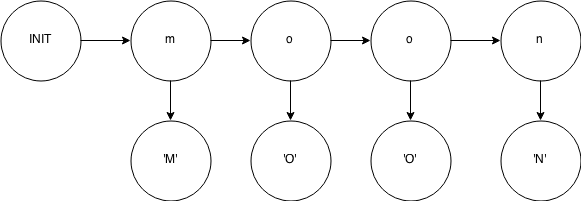
\includegraphics[scale=0.4]{ml_project_hmm.png}
\end{center}
\caption{Hidden markov model for the word "moon". Observed states are the written pixels.}
\label{fig:hmm-letters}
\end{figure}

\section{Related Work}
The first related work we looked at was a similar study by Ivan Dervisevic[1], which utilized four classifiers(Naive Bayes, Complement Naive Bayes, SMO, and C4.5) to perform OCR and compared the results of these classifiers. SMO is a kind of support vector machine classifier while C4.5 is a decision tree classifier. The dataset that was used contained capital characters from 238 TrueType fonts and the data was 40x40 pixel images of each character. In addition to using the raw unprocessed pixel image data, refined datasets with processed representations of the characters were also used. As our focus is more on the machine learning portion and less on the image processing techniques, we will only be using 2 classifiers as a baseline, leaving out image processing, and focusing on implementing a HMM to optimize classification instead.

The second related work we looked at was an introduction to Hidden Markov Models[2] by Rabiner. Since we have not had any comprehensive experience with HMMs, we thought it would be a good idea to see what has already been accomplished with HMMs. In this paper, Rabiner provides a review of the theoretical aspects of using HMMs modeling, and also shows how they apply to machine recognition of speech. This overview serves to provide a good background on the theory and application of HMMs, as well as the limitations that Rabiner discusses in the final section.

\section{Methods}
We selected a few approaches to building classifiers for OCR, including Naive Bayes, Logistic Regression, MLE-learned parameters, Expectation-Maximization (Baum Welch), and Support Vector Machine. After training the classifiers on the training set, we ran the trained classifiers on a test data set for which we know the correct labels, and compared the predicted labels with the correct labels to get the accuracy of the classifiers. Also, we did cross-validation to get a confident accuracy rating for our approaches. 

\section{Experiments}
\subsection{Data Set}
The dataset we are using contains handwritten words. The dataset was collected by Rob Kassel at MIT Spoken Language Systems Group. A subset of the words were chosen and the images of each letter were rasterized and normalized. Since the first letter of each word was capitalized and the rest were lowercase, the first letter was removed and only the lowecase letters were used. The given tab delimited data file  contains a line for each letter, with its label, pixel values, and several additional fields listed in a separate file. 

\begin{figure}[h]
\begin{center}
	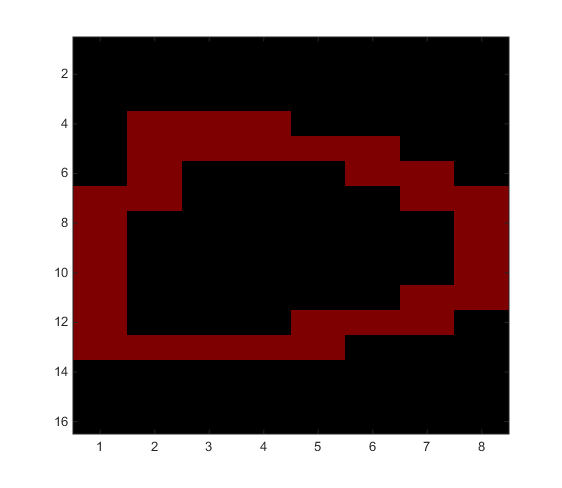
\includegraphics[scale=0.15]{o.png}
	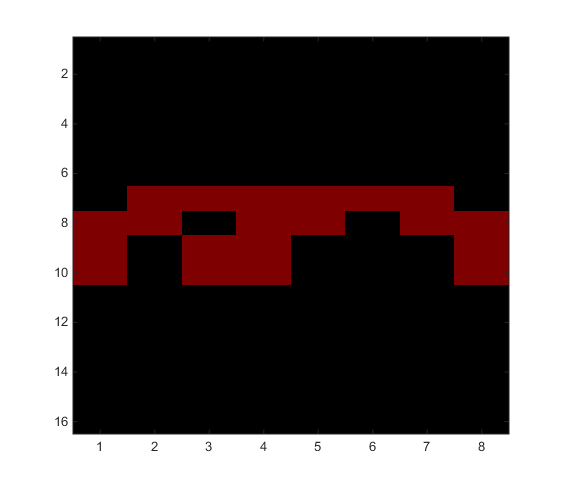
\includegraphics[scale=0.15]{m.png}
\end{center}
\caption{Visualization of two samples in the data set}
\label{fig:dataset-letters}
\end{figure}

Figure \ref{fig:dataset-letters} shows matlab-generated images of the pixel data provided in the data set. The left image is an 'o' and the right image is an 'm'.


The data set can be accessed at \url{http://ai.stanford.edu/~btaskar/ocr/}

\section{Results - Baseline}
\subsection{Naive Bayes}
For our first baseline we performed Naive Bayes on the raw pixel data.
If given some character $c$ and an array of n binary pixel values $\{p_1, ..., p_n\}$, the algorithm is based on basic Bayes rule:
$$P(c|p_1, p_2, ... , p_n) = \frac{P(p_1, p_2, ... , p_n|c)p(c)}{p(p_1, p_2, ... , p_n)}$$
If we make the assumptions that individual pixels are conditionally independent given some character then we can expand the conditional probability in the numerator. Using the naive bayes algorithm in the statistics toolbox for Matlab, we ran Naive Bayes over our dataset consisting of pixel data for 52152 characters(26 unique characters, no capitals) with each observation having 128 binary pixel values.

N-fold cross validation splits the data into N disjoint sets. In each of N iterations training is done on N-1 sets and testing is done on the remaining 1 set. If we take the mean accuracy we can then average out errors resulting from variance.


\begin{table}[h]
\centering
\begin{tabular}{|c|c|c|c|c|c|c|c|c|c|c|c|c|c|c|}
\hline
Iteration & 1 & 2 & 3 & 4 & 5 & 6 & 7 & 8 & 9 & 10 & Avg \\
\hline
Accuracy (\%) & 62.5 & 61.9 & 62.9 & 62.9 & 63.7 & 62.9 & 62.6 & 63.0 & 61.8 & 62.8 & 62.7\\
\hline
\end{tabular}
\caption{Test accuracy of MLE-learned HMM classifier after 10-fold cross validation}
\label{tab:mid-logr-results}
\end{table}

We performed 10-fold cross validation for our Naive Bayes classifier and were able to obtain a final accuracy of 62.7\%.

\begin{figure}[h]
\begin{center}
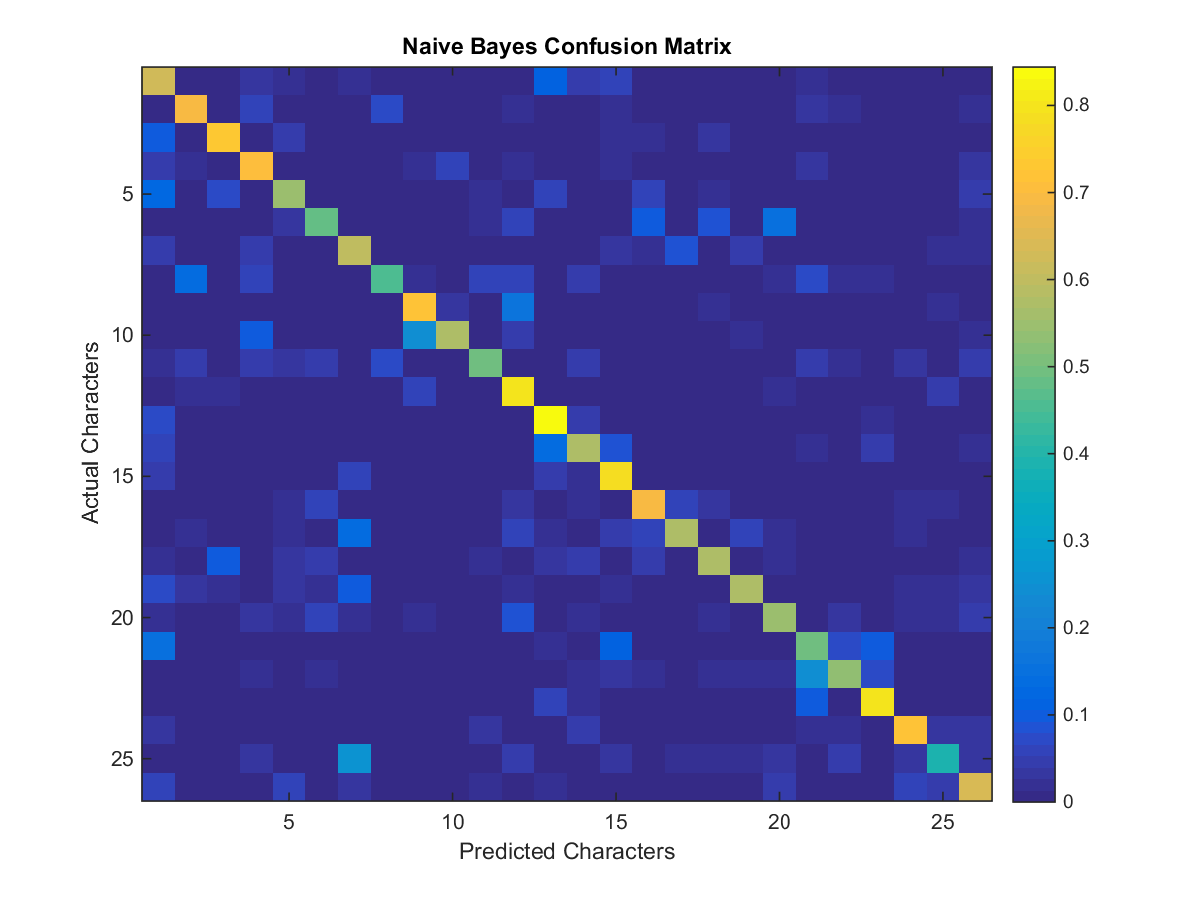
\includegraphics[scale=0.3]{confusion_nb.png}
\end{center}
\caption{Visualization of the confusion matrix for Naive Bayes}
\label{fig:nb-conf-mat}
\end{figure}

Figure \ref{fig:nb-conf-mat} shows a visualization of the confusion matrix obtained from using a trained Naive Bayes classifier to predict a test set of characters. The y-axis shows the actual characters(1 is 'a', 2 is 'b' etc.), while the x-axis shows the predicted characters. The matrix is normalized as such:
$$I_{x, y} = \frac{\mbox{Classified}_{x, y}}{\mbox{Total}_{y}}$$
The value at each coordinate (x,y) is equivalent to the number of instances of character y that has been classified as character x divided by the total instances of character y in the test set. A perfectly yellow diagonal with deep blue everywhere else is thus a representation of a perfect classifier.

From the confusion matrix, some of the commonly misclassified letters are 'h', 'k', 'n', and 'y'. Specifically, looking at row 14, 'n' seems to be commonly misclassified as 'm' or 'o'. 

\subsection{Logistic Regression}
The other classifier that we chose for our baseline is logistic regression.
Logistic regression transforms a given binomial dependent variable, eg. the result of a coin toss, and applies the logistic function to it, effectively transforming it into a continuous variable, as such:
$$F(x) = \frac{1}{1+e^{-(-\beta_0 + \beta_1x)}}$$
The logistic function is useful because it is a function mapping from real numbers to an interval between 0 and 1, and hence the output can be treated as a probability. The logistic regression algorithm itself then follows an approach similar to linear regression to train a set of weight($\beta_0, \beta_1...$) that maximizes the likelihood of the data.

In our case, as we have 26 unique characters which cannot be represented by a binomial variable, we chose to use the multinomial logistic regression algorithm (\texttt{mnrfit}) provided in the statistics toolbox in Matlab. The model takes basically the same principles governing logistic regression for a binary dependent variable, except that it assigns one of the categories for the dependent variable as a 'reference category', and calculates the probabilities of an observation being in each of the other categories as opposed to being in the reference category. For the parameters we used the nominal (default) model, as there is no natural ordering among our response variable categories that would better suit an ordinal model.

When running the logistic regression algorithm, we noticed an abnormally long run time. Hence, we eventually reduced the number of examples in the data to 2000 as well as using principal component analysis to reduce the dimensionality of the data. Even so, there were warnings that the model failed to converge. We suspect that this could be a result of the sparseness of the data matrix as there are a large proportion of 0s' in the data set.

\begin{figure}[h]
\begin{center}
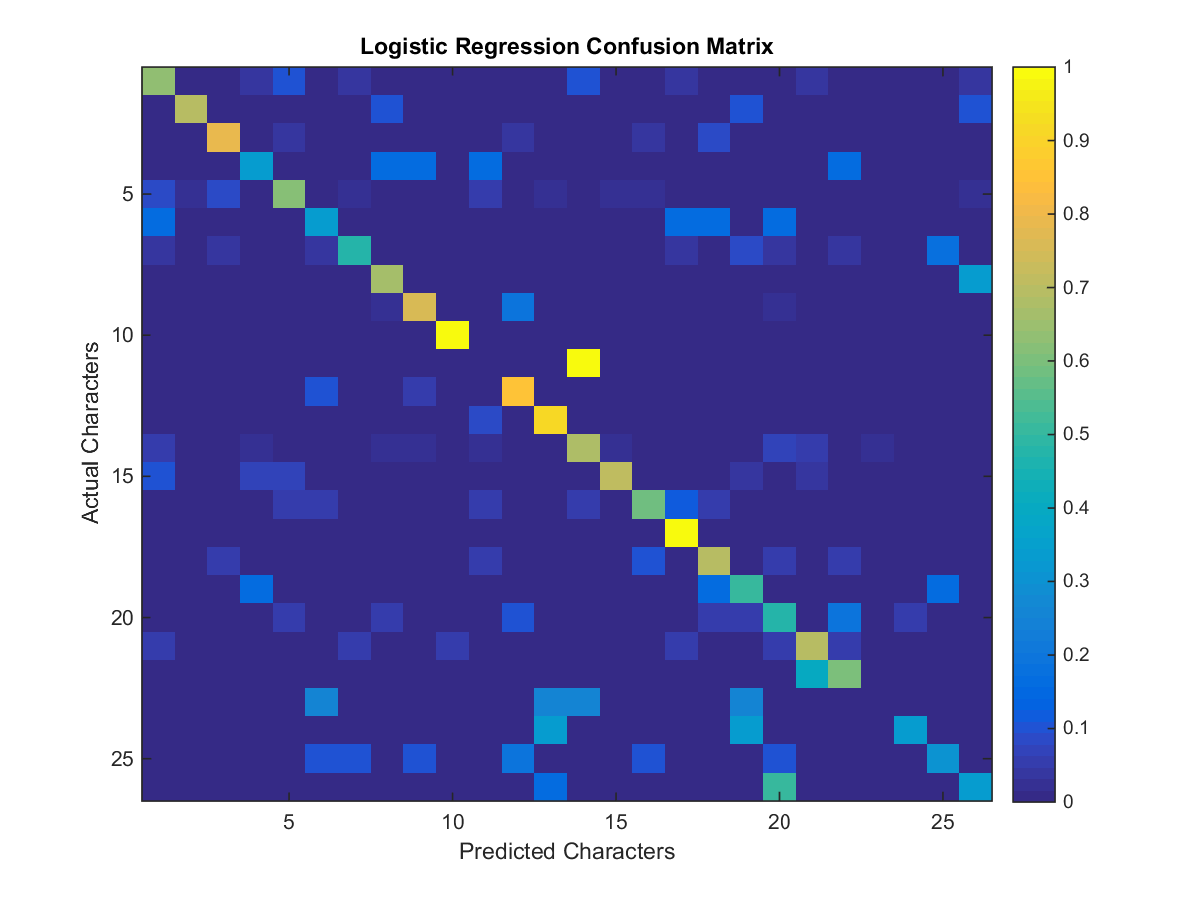
\includegraphics[scale=0.3]{confusion_lr.png}
\end{center}
\caption{Visualization of the confusion matrix for Logistic Regression}
\label{fig:lr-conf-mat}
\end{figure}

Figure \ref{fig:lr-conf-mat} shows the confusion matrix when using a model trained by logistic regression(with 80\% variance retained) to classify a test set. Comparing it to Figure \ref{fig:nb-conf-mat}, it seems like the mistakes that logistic regression are quite different from those made by Naive Bayes. For instance, Naive Bayes was able to classify 'x' and 'z' with fairly high accuracy, but not logistic regression. Furthermore, an interesting fact is that logistic regression seems to get specific characters completely wrong, for instance, classifying 'k' as 'n' in all instances.

\begin{table}[h]
\centering
\begin{tabular}{|c|c|c|c|c|c|c|c|c|}
\hline
Iteration & 1 & 2 & 3 & 4 & 5 & Avg \\
\hline
Accuracy (\%) & 72.00 & 65.75 & 64.50 & 65.25 & 64.75 & 66.45 \\
\hline
\end{tabular}
\caption{Test accuracy of Logistic Regression classifier after 5-fold cross validation}
\label{tab:mid-logr-results}
\end{table}

Table \ref{tab:mid-logr-results} shows the accuracy of a trained logistic regression model in which PCA was performed on a reduced data set with 2000 data points, keeping 70\% of the variance, over 5-fold cross validation. There were significant gains over the Naive Bayes model with an average of 66.45\% accuracy, but the training took a lot longer(Over 20 minutes even with parallel loops) even on the reduced data set with reduced number of features.

We were also curious about how the amount of dimensionality reduction would affect accuracy, and thus did logistic regression on 2000 data points with different extents of reduction(60\%, 70\%, 80\% variance retained), resulting in overall 25, 34, and 49 features respectively, down from 128.

\begin{figure}[h]
\begin{center}
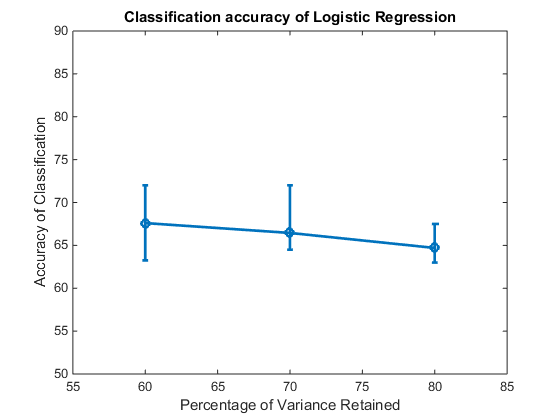
\includegraphics[scale=0.4]{lr_acc.png}
\end{center}
\caption{Logistic Regression Classification with different extent of dimensionality reduction}
\label{fig:lr-dim-red}
\end{figure}

From Figure \ref{fig:lr-dim-red}, it appears that both the variance and accuracy of classification decreased with increasing percentage of variance of the data retained, with 60\% variance retained having the best results. This suggests that perhaps logistic regression is not a very good model for our classification problem as it is not able to make use of more data to improve the model's accuracy.

\section{Results - Intermediate}

\subsection{MLE-Learned HMM Parameters}

We can model a sequence of handwritten letters using a Hidden Markov Model (see Figure~\ref{fig:hmm-letters}). Each hidden state is a letter $c$. Each observed state is a pixel vector $V, v_i \in \{0,1\}$, with length 128 (this is a $16 \times 8$ image). 

To obtain a Hidden Markov Model, we need to find the following parameters:
\begin{itemize}
	\item $\pi_i$ : transition probability from state \texttt{INIT} to $i$
	\item $\phi_{i,j}$ : transition probability from state $i$ to $j$
	\item $\theta_{i}(v)$ : emission probability associated with state $i$ of a pixel vector $v$
\end{itemize}

We plan to use Maximum Likelihood Estimates to find $\phi_{i,j}$. Let $c_1, c_2$ be consecutive letters. Then this is equivalent to finding $P(c_2 | c_1)$. This can be calculated using MLE as follows:
$$ P(c_2 | c_1) = \frac{\mycount(c_1, c_2)}{\mycount(c_1)}$$
We are counting the number of times the bigram $<c_1, c_2>$ appears, and dividing by the number of times $<c_1>$ appears.

To find $\theta_{i}(V)$, we find $P(v | c)$ where $c$ is the letter that is associated with state $i$. Assume Naive Bayes (conditional independence) assumption on $P(v | c)$, so we have 
$$ P(v | c) = \prod_i P(v_i | c)$$
This can be obtained from the training data by looking at all pixel vectors for letter $c$, and applying MLE to calculate $P(v_i = 0 | c)$ and $P(v_i = 1 | c)$ using the frequencies of the pixels that are 0 or 1. In other words,
$$ P(v_i = 1 | c = l) = \frac{\mycount(c = l, v_i = 1)}{\sum_{j=0}^1 \mycount(c = l, v_i = j)}$$

Given $(\pi, \phi, \theta)$, the Viterbi algorithm finds the most likely sequence of hidden states for a HMM that would produce the given sequence of observations. This is done using the bottom-up approach in dynamic programming, and the asymptotic runtime complexity is $O(T|S|^2)$, where $T$ is the length of the observation sequence, and $|S|$ is the number of hidden states.

Given the set of hidden states $S$ with $\pi$, $\phi$, and $\theta$ as described above, as well as the observed pixel vectors $v_1, ..., v_T$, we have the following recurrence relations:
\begin{eqnarray*}
	V_{1,k} &=& \theta_k(v_1) \cdot \pi_k \\
	V_{t,k} &=& \max_{x \in S} \left( \theta_k (v_t) \cdot \phi(x,k) \cdot V_{t-1,x} \right)
\end{eqnarray*}
Let the most likely sequence of hidden states be $c_1, ..., c_T$. We can keep pointers to previous state. Let $\gamma(c_t, t)$ mean the previous state of $c_t$ at iteration $t$. Then,
\begin{eqnarray*}
	c_T = \mbox{argmax}_{x \in S} V_{T,x} \\
	c_{t-1} = \gamma(c_t, t)
\end{eqnarray*}

A word is a sequence of letters $Y = <c_1, c_2, ..., c_n>$ with an accompanying sequence of pixel vectors $V = <v_1, ..., v_n>$, where $n$ is the length of the word. To classify a word, feed the above parameters into the Viterbi algorithm, with the observed states as $v_1, ..., v_n$ to obtain the most likely path of hidden states $\hat{Y} = <c_1, ..., c_n>$, which are the letters. We can then compare the sequence $\hat{Y}$ to the correct labels $Y$ and derive the accuracy of the MLE-learned HMM at OCR.

\begin{table}[h]
\centering
\begin{tabular}{|c|c|c|c|c|c|c|}
\hline
Iteration & 1 & 2 & 3 & 4 & 5 & Avg \\
\hline 
Accuracy (\%) & 69.77 & 70.08 & 67.72 & 70.61 & 70.11 & 69.7 \\
\hline 
\end{tabular}
\caption{Test accuracy of MLE-learned HMM classifier after 5-fold cross validation}
\label{tab:mle-hmm-results}
\end{table}

After 5-fold cross validation, we were able to obtain a mean accuracy of 69.7\% (see Table~\ref{tab:mle-hmm-results}), which is more than 5\% better than either Naive Bayes or Logistic Regression.\\

\begin{figure}[h]
\begin{center}
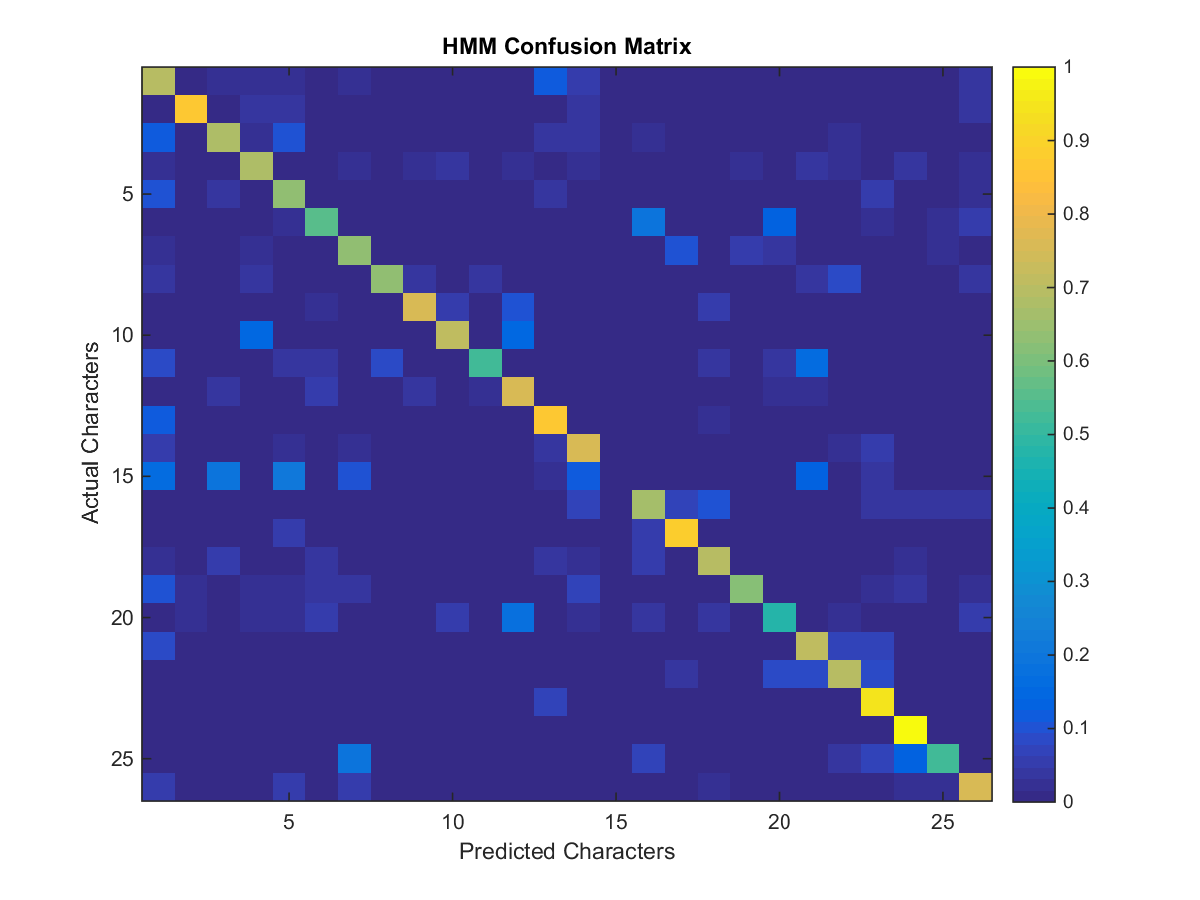
\includegraphics[scale=0.3]{confusion_hmm.png}
\end{center}
\caption{Visualization of the confusion mat for MLE-learned HMM classifier}
\end{figure}

The figure above shows the confusion matrix obtained from using our MLE-learned HMM for classification of a test set. When we compare it to those obtained from Naive Bayes or Logistic Regression, there are some similarities, for instance low accuracy in classifying the character 'y'. Something interesting to note is how much trouble the model has with classifying the character 'o'(row 15), most commonly misclassifying it as 'a', 'c', 'e', 'g', 'n' or 'u', while Naive Bayes does not face the same difficulty. Since the emission probabilities essentially work like Naive Bayes, or a close approximation of it, in this case the transition probabilities we derived may potentially have decreased the classification accuracy instead, in a scenario where the emission probabilities were not certain to begin with, by increasing the uncertainty, since 'o' is a commonly used vowel and does not have as rigid transition rules as consonants.

%\subsection{MLE-Learned HMM Comparison to Baseline}
%
%The mean accuracy of the MLE-learned HMM (69.7\%) is more than 5\% more accurate than either the Naive Bayes classifier (62.7\%) or the Logistic Regression classifier (64.1\%). We theorize that this is because the HMM model accounts for the transitions between letters, hence is more likely to predict a character that, in the training data, has appeared after the previous character.
%
%One of the shortcomings thus far might be the Naive Bayes assumption on the pixel vector, where we assume that the value of each pixel is independent of other surrounding pixels, given the same character. This is unfortunately not true, since a writing instrument is likely to have a line-width of more than 1 pixel. Furthermore, writing often happens in sets of continuous strokes. This implies that if one pixel is switched on, it is more likely that the surrounding pixels are switched on than not.
%
%Another shortcoming is the assumption of the hidden states as being a modeled as per figure ~\ref{fig:hmm-letters}. This assumption lets us use MLE to calculate the transition states. This assumption may result in lower performance, and we will have to wait until we use the Baum-Welch algorithm to estimate the transition and emission probabilities without any assumptions on the hidden states in the learning phase.

\subsection{Filtering +  Naive Bayes}

One thing that caught our attention was the fairly low classification accuracy of the Naive Bayes model. We suspected that one of the main problems with the model is the independence assumption on individual pixels in the same vector. This assumption is not true because we can imagine that even if we knew what some letter was, how the handwritten version appears is not fixed, and is indeed likely to be dependent on values of neighboring pixels. To put this to the test, we came up with a method of applying some filters to the data first and then classifying the processed data with a trained Naive Bayes model.

We used mainly two filters. The first assigned a unique value to each pattern that a given cluster can assume, with two sizes, 3x3 and 4x4, as below. For convenience we will refer to this as the bitstring filter.

\begin{center}

$\left[
\begin{array}{ccc}
2^0&2^1&2^2\\
2^3&2^4&2^5\\
2^6&2^7&2^8\\
\end{array}
\right]$
$\left[
\begin{array}{cccc}
2^0&2^1&2^2&2^3\\
2^4&2^5&2^6&2^7\\
2^8&2^9&2^{10}&2^{11}\\
2^{12}&2^{13}&2^{14}&2^{15}\\
\end{array}
\right]$

\end{center}

Looking at the 3x3 filter, for instance, we see it projects each pixel and its 8 surrounding pixels onto a bit-string of length 9, depending on the values they assume, hence assigning equal importance to all neighbors. 

\begin{table}
\begin{center}
\begin{tabular}{cc}
$\frac{1}{16}*\left[
\begin{array}{ccc}
1&2&1\\
2&4&2\\
1&2&1\\
\end{array}
\right]$ &

$\frac{1}{256}*\left[
\begin{array}{ccccc}
1&4&6&4&1\\
4&16&24&16&4\\
6&24&36&24&6\\
4&16&24&16&4\\
1&4&6&4&1\\
\end{array}
\right]$ \\
\end{tabular}
\end{center}
\end{table}


The second filter we used was a simple gaussian filter that assigned the most importance to the central pixel and then less importance as the distance from the center increased. We will refer to this as the gaussian filter.

\begin{figure}[h]
\begin{center}
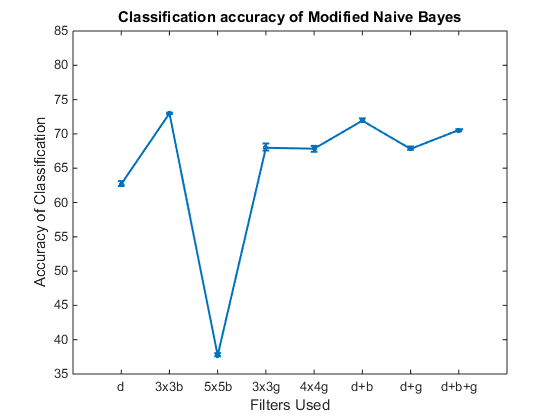
\includegraphics[scale=0.35]{nb_mod.png}
\end{center}
\caption{d=default. b=bitstring. g=gaussian. Combinations use 3x3 filters.}
\label{fig:filter-comb}
\end{figure}

\begin{table}[h]
\centering
\begin{tabular}{|c|c|c|c|c|c|c|}
\hline
Iteration & 1 & 2 & 3 & 4 & 5 & Avg \\
\hline 
Accuracy (\%) & 72.89 & 72.95 & 72.91 & 73.09 & 73.11 & 73.0 \\
\hline 
\end{tabular}
\caption{Test accuracy of Modified Naive Bayes classifier after 5-fold cross validation}
\label{tab:mod-nb-cross-val}
\end{table}

As shown in Table \ref{tab:mod-nb-cross-val}, after 5-fold cross validation, we obtained an average test accuracy of 73.0\%.

Looking at Figure \ref{fig:filter-comb}, We see that all filters attempted except for the 5x5 bitstring filter helped to improve classification accuracy up from the 63\% obtained on the default data. We think that the reason that the 5x5 filter had such bad performance is because the size of the filter is simply too large as compared to the overall size of the character, and hence resulted in too much loss of information. Also, it is noteworthy that the 3x3 bitstring filter had the best performance improvement of close to 10\%, surpassing even the HMM model with MLE estimates, and also did better than the modified datasets containing combinations of filtered data and the default data(sets 6-8 on the x-axis).

\subsection{Support Vector Machine}

Support Vector Machine is a powerful machine-learning algorithm that is able to utilize kernels to find a maximum-margin hyperplane that separate the data points into their respective classes. For our project we use the libsvm toolkit created by Chih-Chung Chang and Chih-Jen Lin[3]. The default soft-margin SVM, given some $n$ training examples, is characterized by the objective function:
$$\mbox{argmin}_{w, \xi, b}\{\frac{1}{2}||w||^2 + C\sum^n_{i=1}\xi_i\}$$
subject to the constraint
$$\forall_i y_i(w\cdot{x_i}-b) \geq 1 - \xi_i$$
where $\xi_i$ is a slack term that allows a data point to trespass the margin, and hence 'soft-margin', and $C$ is a term that controls how much to penalize for a given amount that the margin has been trespassed. We use the soft-margin SVM together with the radial basis kernel function for classifying our data set. The radial basis function is given by the equation:
$$k(x_i, x_j) = exp(-\gamma||x_i\cdot{x_j}||^2), \gamma > 0$$
Hence, we mainly have 2 terms that can be optimized, $\gamma$ and $C$.
We use grid search with 5-fold cross validation to optimize across 5 values of $C$ and 7 values of $\gamma$.\\

\begin{figure}[h]
\begin{center}
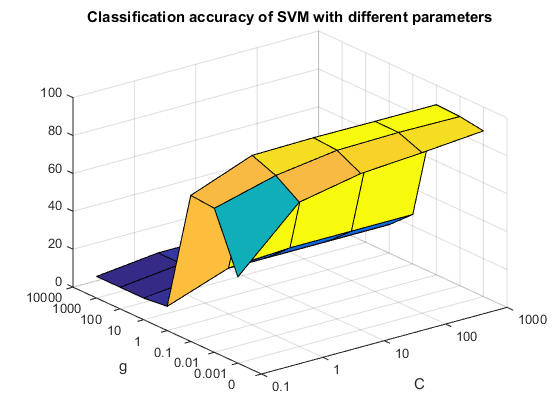
\includegraphics[scale=0.3]{svmview1.png}
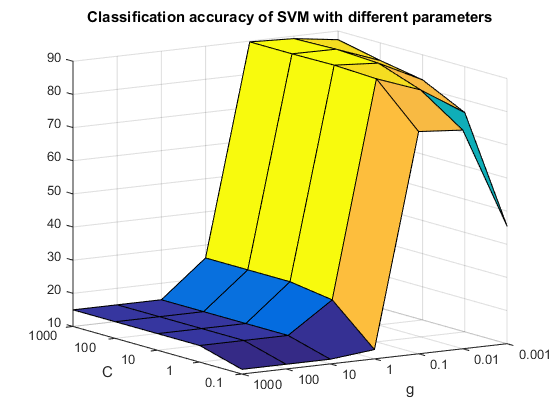
\includegraphics[scale=0.3]{svmview2.png}
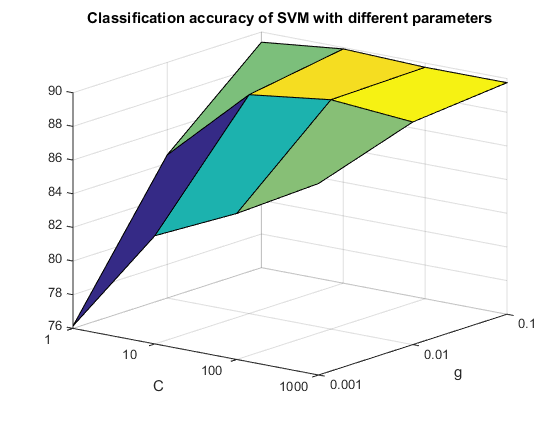
\includegraphics[scale=0.3]{svmview3.png}
\end{center}
\caption{SVM accuracy with different values of $C$ and $\gamma$}
\label{fig:svm-acc-c-gamma}
\end{figure}

From the first 2 graphs in Figure \ref{fig:svm-acc-c-gamma}, we see that values of $\gamma$ larger than 1 contributed sharp decrease in accuracy regardless of the values of $C$, and there seems to be an 'optimal range' of values, shown by the yellow grids, where accuracy hovered around 89\%. After removing the sub-optimal range, we obtain the graph at the bottom of Figure \ref{fig:svm-acc-c-gamma}, which shows our optimal value of $C=10$, $g=0.1$, which was able to obtain a classification accuracy of $89.9\%$ as shown in Table \ref{tab:svm-cross-val}.

\begin{table}[h]
\centering
\begin{tabular}{|c|c|c|c|c|c|c|}
\hline
Iteration & 1 & 2 & 3 & 4 & 5 & Avg \\
\hline 
Accuracy (\%) & 89.92 & 89.94 & 89.97 & 89.59 & 90.16 & 89.9 \\
\hline 
\end{tabular}
\caption{Test accuracy of Support Vector Machine classifier after 5-fold cross validation}
\label{tab:svm-cross-val}
\end{table}

\begin{figure}[h]
\begin{center}
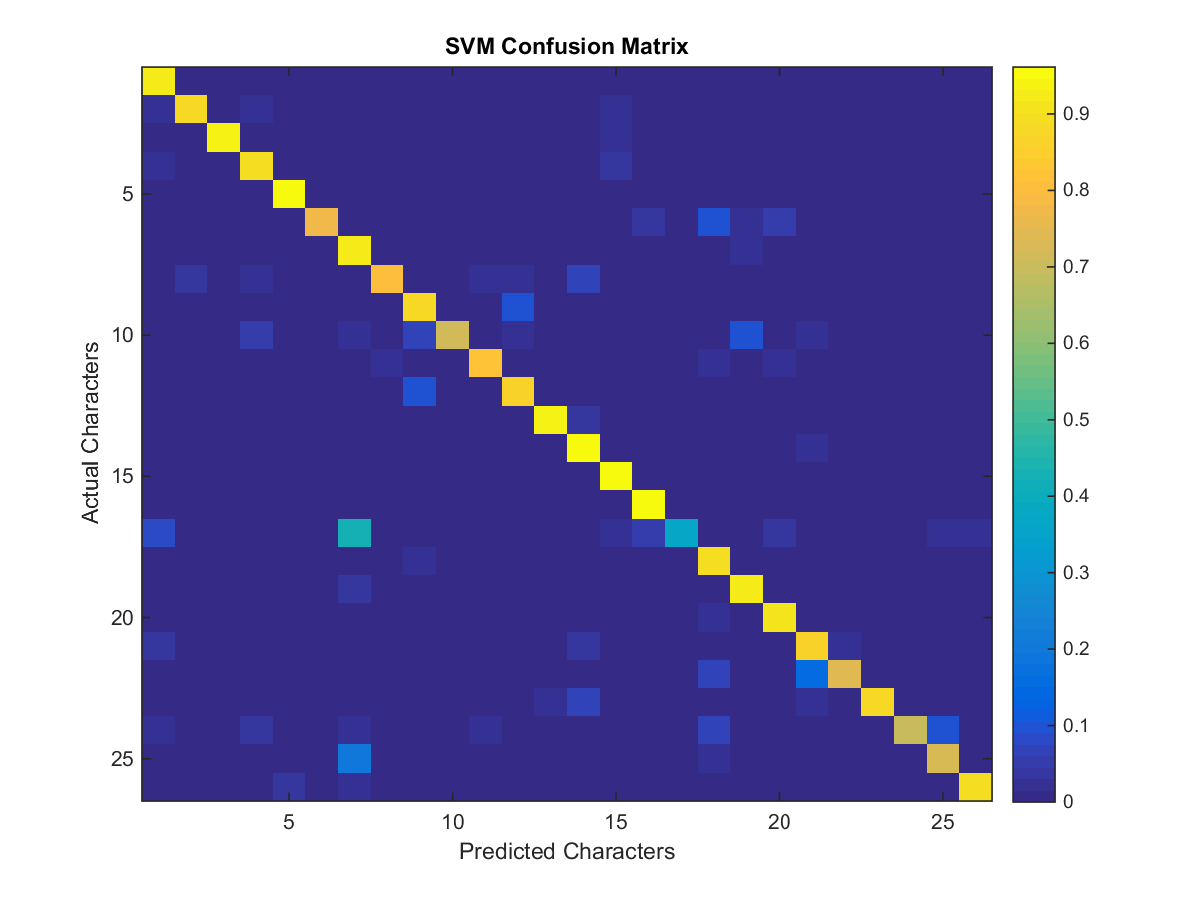
\includegraphics[scale=0.3]{confusion_svm.png}
\end{center}
\caption{SVM confusion matrix}
\label{fig:svm-conf-mat}
\end{figure}

Analyzing the SVM confusion matrix is a lot easier than for the baseline classifiers because of the relatively smaller number of mistakes. Looking at Figure \ref{fig:svm-conf-mat}, there are a few outstanding pairs of classification mistakes, including ('q', 'g'), ('l', 'i'), ('x', 'y'), ('v', 'u'), and ('y', 'g').

\section{Results - Final}

\subsection{Expectation Maximization (EM)}

As part of the final extension, we decided to use the known Baum-Welch algorithm to estimate the parameters of our HMM. The Baum-Welch algorithm iteratively tries to estimate parameters by maximizing the likelihood of the parameters over the observations on each iteration. Each iteration is guaranteed to increase the log-likelihood of the data.

\subsubsection{Brief Algorithm Summary}

A summary of the Baum-Welch algorithm is as follows[4]. Let $X = {x_1, ..., x_T}$ be the sequence of observations, $Z = {z_1, ..., z_N}$ be the set of hidden states, $A = \{ a_{ij} \}$ where $a_{ij} = \phi_{i,j}$. $B = \{ b_j(x) \}$ where $b_j(x) = \theta_i(x)$. Redefine $\theta$ as the set of parameters to optimize, where $\theta = (A, B, \pi)$. Seed $\theta$ with initial conditions (e.g. random).

The forward procedure involves calculating $\alpha_i(t) = P(x_1, ..., x_t, Z_t = i | \theta)$. This is the probability, at time $t$, of being in state $i$ and having seen observations $x_1, ..., x_t$. 

The backward procedure involves calculating $\beta_i(t) = P(x_{t+1}, ...,x_T, Z_t = i | \theta)$. This is the probability, at time $t$, of being in state $i$ and then seeing observations $x_{t+1}, ...,x_T$ in the future. 

The forward and backward procedures can be used to evaluate $\gamma(z_n)$ and $\xi(z_{n-1},z_n)$, which is used to complete EM as described in Section 13.2.1 of Bishop[4].

\subsubsection{Test Results}

We seeded $\theta$ of the Baum-Welch algorithm with the MLE estimates obtained earlier. We removed the labels on each character, and assuming conditional independence on the pixels (emulating a Dynamic Naive Bayesian Classifier [5]) used the pixel vectors as the observation sequence for Matlab's \texttt{hmmtrain} function.

\begin{table}[h]
\centering
\begin{tabular}{|c|c|c|c|c|c|c|}
\hline
Iteration & 1 & 2 & 3 & 4 & 5 & Avg \\
\hline 
Accuracy (\%) & 65.19 & 65.84 & 66.52 & 68.18 & 65.78 & 66.3 \\
\hline 
\end{tabular}
\caption{Test accuracy of EM learned HMM classifier after 5-fold cross validation}
\label{tab:bw-cross-val}
\end{table}

We noted that there was a deprovement in accuracy compared to the original MLE-learned HMM classifier we experimented with earlier. After 5-fold cross validation, we obtained a test accuracy of 66.3\% as shown in Table \ref{tab:bw-cross-val}. This is about 3\% lower than that of the MLE-learned HMM classifier. Considering the possibility that the MLE estimates do not provide the best prior for $\theta$, we tried using random values for $\theta$, but these produce worse accuracies.

We theorize that although the Baum-Welch algorithm works well for discrete observations, this does not fit well in the case where pixel vectors are the observations. Each hidden state produces 128 different binary observations (pixel values of \textbf{on} or \textbf{off}). Furthermore, although pixels are clearly not conditionally independent, we had to assume this to run the algorithm.

\subsection{HMM + SVM}

As the last method to try to improve the OCR test accuracy, we decided to combine the results of the SVM classifier with the MLE-learned HMM. A new set of parameters were derived in the following way:
\begin{enumerate}
	\item $\pi_i$, $\phi_{i_j}$ : Use the same initial transition probabilities as in the MLE-learned HMM classifier
	\item $\theta_c(V)$ : Use the probability $P(Y=c|V)$ given by the SVM classifier, where $Y$ is the random variable denoting the hidden state (the letter), $c$ is the hidden state corresponding to letter '$c$', and $V = <v^{(1)}, ..., v^{(128)}>$ is the $16 \times 8$ pixel vector
\end{enumerate}
The justification for 2. is as follows. $\theta_i(v)$ is $P(V|Y=c)$, that is, the probability of emitting the pixel vector $V$ given that we are currently in state $c$. By Bayes theorem, 
\begin{eqnarray*}
	P(V|Y=c) &=& \frac{P(Y=c|V)P(V)}{P(Y=c)} \\
	&\propto & P(Y=c|V) \\
\end{eqnarray*}
The SVM classifier is able to produce a list of probabilities $P(Y = c | V)$ for each  $c \in \{'a', 'b', ..., 'z'\}$, so to find $\theta_i(V)$, we simply classify $V$ using the SVM classifier and pick the value corresponding to $c$.

\subsubsection{Test Results}

\begin{table}[h]
\centering
\begin{tabular}{|c|c|c|c|c|c|c|}
\hline
Iteration & 1 & 2 & 3 & 4 & 5 & Avg \\
\hline 
Accuracy (\%) & 91.64 & 91.61 & 92.38 & 92.00 & 90.11 & 91.5 \\
\hline 
\end{tabular}
\caption{Test accuracy of HMM + SVM classifier after 5-fold cross validation}
\label{tab:hmm-svm-cross-val}
\end{table}

As shown in Table \ref{tab:hmm-svm-cross-val}, after 5-fold cross validation, we obtained an overall accuracy of 91.5\%. This is highest accuracy we were able to obtain thus far.

We think that this procedure combines the merits of Support Vector Machines and Hidden Markov Models, hence producing the best performance. The SVM classifier produces a reliable estimate of $P(Y=c|V)$ without having to assume conditional independence of the individual pixels. The HMM takes into account that certain state (i.e. letter) transitions are much more likely than others due to the fact that English words are not made up of random letters.

\section{Conclusion}

\begin{table}[H]
\centering
\begin{tabular}{|c|c|c|c|c|c|c|}
\hline
ML Technique & Avg Accuracy (\%) \\
\hline 
Naive Bayes & 62.7 \\
Logistic Regression & 66.5 \\
\hline 
MLE-learned HMM & 69.7 \\
Filtering + Naive Bayes & 73.0 \\
SVM & 89.9 \\
\hline 
EM (Baum-Welch) & 66.3 \\
SVM + HMM & 91.5 \\
\hline 
\end{tabular}
\caption{Summary of ML techniques applied to OCR and their accuracies}
\label{tab:summary-ml-tech}
\end{table}

Table \ref{tab:summary-ml-tech} shows a summary of the Machine Learning techniques applied to solve the problem of Optical Character Recognition. As baselines, we applied a Naive Bayes and Logistic Regression classifier, which produced mediocre results. Next, we tried using MLE-learned HMM parameters with the Viterbi algorithm, producing slightly better results. We also experimented with feature engineering, applying filters to the pixels before training the Naive Bayes classifier. Finally, we discovered that SVM does extremely well in classifier letters independently. When SVM was combined with the MLE-learned HMM parameters and fed as input to the Viterbi algorithm, we produced the highest accuracy of 91.5\%.

\subsubsection*{References}

\small{
[1] Ivan Dervisevic(2006) {\it Machine Learning Methods for Optical Character Recognition.} \url{http://perun.pmf.uns.ac.rs/radovanovic/dmsem/complete/2006/OCR.pdf}

[2] Lawrence R. Rabiner (1989) {\it A Tutorial on Hidden Markov Models and Selected Applications in Speech Recognition} \url{http://www.ece.ucsb.edu/Faculty/Rabiner/ece259/Reprints/tutorial\%20on\%20hmm\%20and\%20applications.pdf}

[3] Chang, Chih-Chung and Lin, Chih-Jen (2011) {\it LIBSVM: A library for support vector machines } \url{http://www.csie.ntu.edu.tw/~cjlin/libsvm}

[4] Christopher M. Bishop (2006) {\it Pattern Recognition and Machine Learning} pp616-624

[5] H.H. Avilés-Arriaga*1, L.E. Sucar-Succar2, C.E. Mendoza-Durán3, L.A. Pineda-Cortés (2011) {\it A Comparison of Dynamic Naive Bayesian Classifiers and Hidden Markov Models for Gesture Recognition} p86 \url{http://www.revistas.unam.mx/index.php/jart/article/view/25279}

}
\end{document}
